% The document class supplies options to control rendering of some standard
% features in the result.  The goal is for uniform style, so some attention 
% to detail is *vital* with all fields.  Each field (i.e., text inside the
% curly braces below, so the MEng text inside {MEng} for instance) should 
% take into account the following:
%
% - author name       should be formatted as "FirstName LastName"
%   (not "Initial LastName" for example),
% - supervisor name   should be formatted as "Title FirstName LastName"
%   (where Title is "Dr." or "Prof." for example),
% - degree programme  should be "BSc", "MEng", "MSci", "MSc" or "PhD",
% - dissertation title should be correctly capitalised (plus you can have
%   an optional sub-title if appropriate, or leave this field blank),
% - dissertation type should be formatted as one of the following:
%   * for the MEng degree programme either "enterprise" or "research" to
%     reflect the stream,
%   * for the MSc  degree programme "$X/Y/Z$" for a project deemed to be
%     X%, Y% and Z% of type I, II and III.
% - year              should be formatted as a 4-digit year of submission
%   (so 2014 rather than the accademic year, say 2013/14 say).

\documentclass[ % the name of the author
                    author={Samuel Russell},
                % the name of the supervisor
                supervisor={Prof. Bogdan Warinschi},
                % the degree programme
                    degree={MEng},
                % the dissertation    title (which cannot be blank)
                     title={Innocuous Ciphertexts},
                % the dissertation subtitle (which can    be blank)
                  subtitle={The DE-CENSOR Scheme},
                % the dissertation     type
                      type={research},
                % the year of submission
                      year={2018} ]{dissertation}

\usepackage{amsmath}
\usepackage{amsfonts}
\usepackage{amssymb}
\usepackage{hyperref}
\usepackage{parskip}
\usepackage[subrefformat=parens]{subcaption}
\usepackage{pgfplots}
\pgfplotsset{width=7.2cm,compat=1.16}
\usepackage{sidecap}
\usepackage{wrapfig}
\usepackage{multirow}
\usepackage{tabularx}

%\usepackage{lineno}
%\linenumbers

\begin{document}


% =============================================================================

% This macro creates the standard UoB title page by using information drawn
% from the document class (meaning it is vital you select the correct degree 
% title and so on).

\maketitle

% After the title page (which is a special case in that it is not numbered)
% comes the front matter or preliminaries; this macro signals the start of
% such content, meaning the pages are numbered with Roman numerals.

\frontmatter

% This macro creates the standard UoB declaration; on the printed hard-copy,
% this must be physically signed by the author in the space indicated.

\makedecl

% LaTeX automatically generates a table of contents, plus associated lists 
% of figures, tables and algorithms.  The former is a compulsory part of the
% dissertation, but if you do not require the latter they can be suppressed
% by simply commenting out the associated macro.

\tableofcontents


% The following sections are part of the front matter, but are not generated
% automatically by LaTeX; the use of \chapter* means they are not numbered.

% -----------------------------------------------------------------------------

\chapter{Executive Summary}

My research hypothesis is that statistical methods could be used by network based adversaries to distinguish between the use of format transforming encryption schemes and normal traffic. I also hypothesis that an practical replacement scheme will be able to produce innocuous ciphertexts whose distribution has undetectable divergence from the distribution of normal traffic.

\subsubsection{Research Goals}

\begin{itemize}
\item Critically discuss the downfalls of using an FTE system to encode ciphertexts.
-\item Build a statistical tool for distinguishing emulated from normal traffic.
-\item Build a new scheme that is able to overcome this detection.
\end{itemize}

\vspace{1cm} 
{\bf A compulsory section, of at most $1$ page} 

\noindent
This section should pr\'{e}cis the project context, aims and objectives,
and main contributions (e.g., deliverables) and achievements; the same 
section may be called an abstract elsewhere.  The goal is to ensure the 
reader is clear about what the topic is, what you have done within this 
topic, {\em and} what your view of the outcome is.

The former aspects should be guided by your specification: essentially 
this section is a (very) short version of what is typically the first 
chapter.  Note that for research-type projects, this {\bf must} include 
a clear research hypothesis.  This will obviously differ significantly
for each project, but an example might be as follows:

\begin{quote}
My research hypothesis is that a suitable genetic algorithm will yield
more accurate results (when applied to the standard ACME data set) than 
the algorithm proposed by Jones and Smith, while also executing in less
time.
\end{quote}


% -----------------------------------------------------------------------------

\chapter*{Definitions and Acronyms}

\vspace{1cm} 


\begin{quote}
\noindent
\begin{tabularx}{\textwidth}{ r c X }
AES                 &:		& Advanced Encryption Standard                                         \\
DES                 &:		& Data Encryption Standard                                             \\
Normal distribution &:		& Laplace-Gauss distribution
\\
normal traffic		&:		& Traffic generated from a normal person
browsing their normal sites on their normal web browser.\\
FTE					&:		& Format Transforming Encryption\\
DE-CENSOR			&:		& Distribution Encoding of Ciphertexts to Emulate Normal Surfing for Onion Routing\\
Record Layer		&:		& Layer in the network stack that receives data from te application layer, encrypts it, fragments it to an appropriate size and sends it on to the Transport Layer.\\
SOCKS				&:		& Socket Secure - Internet Proxy Protocol

\end{tabularx}
\end{quote}

% -----------------------------------------------------------------------------

\chapter*{Acknowledgements}

{\bf An optional section, of at most $1$ page}
\vspace{1cm} 

\noindent
It is common practice (although totally optional) to acknowledge any
third-party advice, contribution or influence you have found useful
during your work.  Examples include support from friends or family, 
the input of your Supervisor and/or Advisor, external organisations 
or persons who  have supplied resources of some kind (e.g., funding, 
advice or time).
% =============================================================================

% After the front matter comes a number of chapters; under each chapter,
% sections, subsections and even subsubsections are permissible.  The
% pages in this part are numbered with Arabic numerals.  Note that:
%
% - A reference point can be marked using \label{XXX}, and then later
%   referred to via \ref{XXX}; for example Chapter\ref{chap:context}.
% - The chapters are presented here in one file; this can become hard
%   to manage.  An alternative is to save the content in seprate files
%   the use \input{XXX} to import it, which acts like the #include
%   directive in C.

\mainmatter

% -----------------------------------------------------------------------------

\chapter{Motivations}
\label{chap:context}

Tim Berners-Lee said that since its conception, the World Wide Web has been built with the principles of openness and privacy~\cite{gard}. These key values, that also lie at the heart of democracy, can ensure that if a website is made available on web, anyone can connect to it - no matter who they are or where they live. 

However, recently, policies have been made which challenge this status quo; certain content on the internet is now subject to censorship laws in some places like the United Kingdom or China. The motivations behind this censorship can be well-meaning, for example, the blocking of illegal content such as child pornography with the intention of protecting the innocent lives of children. A further attempt to reduce damage to people's lives was the implementation of search engine de-listing of personal content petitioned by the right-to-be-forgotten movement~\cite{rtbf}. However, this decision sparked much controversy since people believed that this deletion of history could lower the quality of the internet. 

However, other cases of censorship are on a much larger scale and are not universally accepted as positive. One example is certain nation states blocking access to content that they deem to be inciting opposition to their political standpoints. This can involve blanket restrictions to foreign websites or restricting sites which may be hosted inside the nation, but are deemed to perpetuate negative views. Many countries ban hate-speech, or exclude it from their freedom of speech laws~\cite{hate} and some countries have Libel rules~\cite{libel} which ban spreading of false information. However, there are a number of nations that actually hide information about certain world events or ideologies from their citizens, depriving their civil rights~\cite{chincensor}. This is dangerous for the world as it creates environments that can breed hatred directed at whomever the censors wants.

There is no doubt that the western economy and society has benefited greatly from the success of the web and its ability to connect people and share information. What ensures the web's success is its status as a permissionless space that leads to creativity, innovation and freedom of expression. This allows any new, small start-up companies and individuals to use this commodity to build services and communities without the need for legal approval or business deals, leaving their projects to be free to grow and prosper. Proposed Net Neutrality regulations would allow internet service providers to prioritise certain site's traffic. This does not permit full censorship but even the slowing down of traffic could reduce the usability of certain sites so that users would avoid them. This would fundamentally coerce browsing person's behaviour to direct them away from certain topics.

Taking an existing example; in China, which is a state with among the most stringent internet censorship practices, the American Chamber of Commerce~\cite{amcham} says that four out of five of its member companies report a negative impact on their business from Internet censorship. This gives financial incentives to ensure the internet remains open.

\section{Network Surveillance and Censorship}

I will categorise censorship in two ways. The first kind is entities on the internet such as websites taking down content. This is most poignant when the content has been made by others, such as on a micro-blogging site like Facebook. Although this is an issue and currently there is debate about the balance of such censorship on these social media platforms, this is not what I will be looking at. This is because the data is gone rather than being blocked. Of course, there are tools that archive content that may be be later retracted or deleted such as The Internet Archive's project: Wayback Machine~\cite{wb}, and access to these resources is what the second type of censorship is about.

Informally, the internet consists of each party's computer equipment connected together with a network of wires (and other mediums) and some management machinery to route communications to their destination.
Communications are packet based and are directed along the connections according to the Internet Protocol (IP)~\cite{ip4}.
This protocol header defines the destination of the packet for the purposes of determining the most appropriate route to follow.
It also contains the address of the source so that error messages can be directed, to the right place, appropriately.
Among other information, like version numbers and flags, there is also a field that tells the intermediary machinery when to delete the message, but this is only for cases where the destination in unreachable. 

The second type of network surveillance and censorship sits at these intermediate points in the network and deals with how these packets are handled. By default, IP, and the transport layer on top of it (TCP), does not encrypt or sign the payload data. Therefore, it is possible for the intermediary parties to read and tamper with the packets and their payloads before they are sent or even dropped from the network. 

From their observations of the Chinese internet filtering systems, Zittrain and Edelman deduced several methods that were being used~\cite{edelman2005empirical}.
Filtering on the IP address of a resource can be done by analysing the destination field of the packet. This is good for blocking direct access to static sites since it  is one of the simplest and therefore fastest to implement, though it relies on comprehensive black or white listing coordination.

The most common method of blocking is for the routers to drop these black-listed packets, but as Clayton et al. found in their practical experiments~\cite{clayton2006ignoring}, for protocols that communicate in a streaming fashion over time, the network machinery sends TCP reset packets to both parties to interrupt the session and stop communication. This type of attack can be easily countered by ignoring all reset packets since, due to how the system is architectured, the original packets are allowed through. They also observed a less frequent technique which was the injection of a forged packet with random synchronisation numbers. When this reaches the destination, the server detects the incorrect value and validly triggers the sending of a reset packet. Now, if the reset packets are ignored then the two real endpoints become out of sync and the communication breaks down. Luckily, as it stands, the forged packets are poor imitations and so are easily detectable.

Another method used in practice is DNS poisoning, which involves incorrectly resolving URLs to redirect users either to a censorship notice or just a random - and useless - address. This only affects the use of URLs and so the use of raw IP address is completely unaffected, although many sites use them internally so it creates difficulty and work for users through setting up of a local host file.

Finally, packet inspection has become very common place. This can be content based detection such as searching for trigger words in HTTP request paths, or in the HTML content returned. A good example of this is search terms included the query parameters of  search engine requests. Although these snooping attacks only apply to clear unencrypted HTTP traffic and using an encrypted  TLS transport layer hides all this information, sites that do encrypt, risk having the whole site IP blocked as above. This happened to Wikipedia in China when the site switched to enforcing HTTPS on all traffic. When the site did this, the Golden Shield Project - in charge of China's network surveillance - could no longer selectively block the specific culprit pages, instead, a blanket ban on the service was enforced.

The packet inspection and classification is also done on a protocol basis. Censors are usually tolerant to users accessing webpages over HTTP or video calling over VOIP protocols, however, protocols that allow the transfer of data in a opaque way such as VPN tunnelling, The Onion Router and TLS (less so) are often blocked completely.

\section{The Onion Router}

One of the most effective tools for evading network surveillance is The Onion Router (TOR) which not only hides the contents of packets like TLS, but also obfuscates their destination. It does this by maintaining a opaque network which decorrelates the movement of packets in and out. As a result, it is hard to work out where traffic that enters the network at an entry node will exit, and then therefore what its final destination is. To realise this, each packet is encrypted three times (on top of standard TLS encryption) and, as the packet moves through the network, a layer of encryption is removed at each relay node. This means, as it mixes with other packets, it is hard to identify and match what is arriving with what is sent on. Paths through the network are randomly allocated and keys are exchanged securely using a Diffe-Helman protocol. This is done one node at a time through the existing link such that nodes only know the identities of their predecessor and successor in the chain. 

However, there has been a lot of work and success around de-anonymising the TOR protocol to gather information on users. There has been research into both passive and active attacks giving varying levels of success but with varying levels of effort. Website fingerprinting attacks such as Cair et al.~\cite{webfinger} only need to eavesdrop at a single point but suffer from a high number of false positives. Traffic confirmation attacks, which require access to both ends of the communication, such as Shmatikov et al.~\cite{conf} need long periods to gain statistical significance. Active attacks, such as water marking through delays, are a lot quicker but they involve a lot more work for the attacker. However, government bodies with large powers such as the NSA are interested in this field, so use of these attacks is not out of the realms of possibility. Even so, if an adversary only controls a small proportion of the network, the chances of being allocated a fully comprised relay chain is small. Recently, Arp et a.~\cite{torben} released a side-channel attack for TOR which is more reliable but less intrusive that other methods that use browser exploits. In fact in their research, Nithyanand et al.~\cite{AS} found that very high levels of active circuits were potentially vulnerable to state level adversaries. To counter this, they have built a TOR client that is aware of adversaries and is able to more intelligently select relay paths. This is successful in reducing the rate of affected connections but, as with all these anonymising techniques, sacrifices performance, adding latency to the circuit generation before any data can be sent.

Although TOR has these issues, it makes the surveillance of users' browsing astronomically harder and so censors such as the Chinese Government have resorted to a complete ban on the protocol. Originally, TOR packets were very recognisable due to their predictable size and structure but some improvement have been made to adjust its fingerprint to match TLS as much as possible. However, more had to be done.

Tor works by allowing users to connect to one of the publicly known entry guard relays. However, since these IP addresses are publicly known, they are easily detected and interfered with by network censor systems. As mentioned, one way this is done is by sending reset packets to both parties telling them to close the TCP stream.
To circumvent this, users instead connect to private bridges in uncensored zones - such as the United States - so that the indented destination of the packets is hidden. However, with protocol fingerprinting by deep packet inspection (DPI) and the use of active probes, censors can still catch these unlisted bridges in under fifteen minutes of use!
The use of obfuscation and FTE (described in section \ref{sec:FTE}) bridges have been able to fool these DPI systems for now since they fool the common protocol classification systems which use regular expressions. However, as deep learning becomes more prevalent it is known that this will not be enough.

\section{Summary}

In this chapter I have explained how there are motivations for wanting to access online resources  with out the controllers of the network being able to determine the content of what you are accessing. I have discussed TOR's roll in this but that access to the TOR network is limited and that even TOR bridges are vulnerable since the traffic patterns are identifiable as TOR. Therefore, there is a need for encodings that cause misclassification of TOR traffic to other innocuous protocols. 

% -----------------------------------------------------------------------------

\chapter{Cryptographic Background}
\label{chap:technical}

After language was invented to share knowledge, humans soon needed a way hide it from those whom it was not intended. The first schemes used word or letter substitutions or the shuffling of characters to make the meaning of a message hard to obtain. These techniques are still used as the basic building blocks today; for example in the AES block cipher, a very popular encryption scheme, of which there are hardware implementations baked in to many of the major computer chips. Early schemes however, relied on the secrecy of the method to protect the privacy of the message which meant that they cannot be reused by others. This lead to the introduction of parametrised constructions that use a key to alter the encryption such as the Vigen\`ere cipher. Modern schemes obey Kerkoff's principle; that the security of the system only depends on the security of the key, allowing the same encryption method to be used by all.
\begin{itemize}
 \item security through obscurity
 \item perfect security - information-theoretic
 \item conditional security
 \item ciphertexts - formatting
 \item block ciphers
\end{itemize}

\begin{itemize}
 \item hiding existence
 \item stenography
 \item honey encryption
 \item deniable encryption
\end{itemize}

% -----------------------------------------------------------------------------

\chapter{Project Execution}
\label{chap:execution}

\section{Format Preserving Encryption}

In 1981, NIST~\cite{FIPS74} outlined a mode of DES that was able to restrict the ciphertext of an encryption to a string of a fixed, finite alphabet such as decimal digits $ \Sigma = \{0,1...9\} $. This allows plain texts such as phone numbers of form $ X \in \Sigma^N $ to be encrypted to a ciphertext $ Y = \Sigma^N $ that is also a phone number. Although that FIPS document is now withdrawn, it sparked further work such as what was done by Brightwell and Smith~\cite{DPE}. They first specify the particular use case of encrypting data in place as inside a database where the ciphertexts must abide by the same type constraints of the database schema. The paper then goes on to describe their  Datatype-Preserving Encryption scheme that again works with DES in a streaming mode and works over an indexed finite alphabet. However the algorithm has redundant elements, such as shuffling the alphabet's ordering, that are not backed up with reasoning and there is no proof of security. More recently, Black and Rogaway~\cite{CAFD} provide three constructions in their paper. They analyse the security of each one against the standard adversary $Adv^{prp}$ and also discuss the practical considerations of scaling asymptotically and in practice.

The field has become a highly practical one, with companies such as Voltage moving to take advantage of the concept. They are using it to upgrade older systems by adding a layer of security that is invisible to the applications that sit on top since does not change the structure of the data. Therefore this vastly reduces the costs of this retrofitting since the need to completely redesign the system is usually eliminated. As of 2018, HPE~\cite{hp} are still pushing it as part of their SecureData product to help maintain legacy software.

To keep up with the work in industry, Bellare et al. wrote a comprehensive paper~\cite{fpe} that formally defines the goals of FTE. They did this in the form of adversary based games. They redefine the standard Pseudo Random Permutation (PRP) Security game which challenges an adversary to distinguish the encryption scheme from a random permutation. The paper also gives weaker notions they think are more appropriate. Single Point Indistinguishably (SPI) requires the adversary to be unable to distinguish between the encryption of any chosen plaintext from the specified language and a randomly selected ciphertext of the same language. The Message Recovery (MR) game gives the adversary the frequency distribution of plaintexts and asks for a decryption of a the ciphertext of a randomly selected item from the plaintext space. The adversary is given adaptive access to an encryption and verification oracle. Finally they define Message Privacy (MP) as the inability of an adversary to compute a function of a plaintext given the ciphertext; Note in this game the adversary can select the function it hopes it will have most success with. They state the following strength hierarchy for these games, showing PRP does give us the Message Recovery property we ultimately want.
$$ PRP \implies SPI \implies MP \implies MR $$
The first implication is trivial since a random function will produce a random element when given the message. The last implications is also trivial since MR is just a special case of MP - where the function is fixed to be the identity. For the proof of $ SPI \implies MP $ the paper shows how an adversary $B$ for SPI can be constructed using an adversary $A$ for MP with sufficiently large advantage. In this construction $B$ is able to run $A$ and satisfy it's calls to the encryption oracle using its own oracle in turn.

\subsection{Rank and Encrypt}

In the second half of the paper~\cite{fpe} Bellare et al. then proposed a framework called Rank then Encipher. This framework supports and enhances the methods already discussed since it enables any encryption scheme that supports arbitrary size alphabets to be used to encrypt more complex languages. It simplifies the complexity of language features such as a checksum character, by mapping words to an simple index so that the encryption scheme used can be generic. It does this by partitioning the language in to slices, each containing the words of a given length. That is, for the language $\mathcal{X} = \{\mathcal{X}_N : N \in \mathcal{N} \}$ for lengths in $\mathcal{N}$, each slice $\mathcal{X}_N = \{ X : X \in \mathcal{X}, \vert X \vert = N  \}$. Now the elements in each slice can be arbitrarily ordered as $\mathcal{X_N} = \{ X_0, X_1, \cdots , X_{n-1} \} $ and a bijective mapping can be defined $rank_N :: \mathcal{X}_N \rightarrow \mathbb{Z}_n$.
Then for the whole language, we can define
$$ rank :: \mathcal{N} \times \mathcal{X} \rightarrow \mathbb{N} \cup \bot $$
$$ rank(N,X) =
\left\{
	\begin{array}{ll}
		rank_N(X)  & \mbox{if } \vert X \vert = N\\
		\bot & \mbox{otherwise} 
	\end{array}
\right.
$$

$$ unrank :: \mathcal{N} \times \mathbb{N} \rightarrow \mathcal{X} \cup \bot $$
$$ unrank(N,i) =
\left\{
	\begin{array}{ll}
		rank_N^{-1}(i)  & \mbox{if } i \in \mathbb{Z}_{\mathcal{X}_N}\\
		\bot & \mbox{otherwise} 
	\end{array}
\right.
$$

Then if we have an encryption scheme $Enc :: \mathcal{K} \times \mathcal{N} \times \mathbb{N} \rightarrow \mathbb{N}$ that works over arbitrary domains to encrypt values into $\mathbb{Z}_{|\mathcal{X}_N|}$, we can define our scheme $\mathcal{E}_k^N = unrank_N \cdot Enc_k^{|X_N|} \cdot rank_N$. Using this construction, they state how the security properties of the original encryption scheme, over the finite domain, is inherited by the the rank then encrypt scheme over the language.

They provide a ranking and un-ranking algorithm for regular languages inspired by the work done by Goldberg in '85~\cite{rank}, but to make this efficient, pre-computation is needed. For each word length, a table of path numbers has to be created which can be done through dynamic programming.

Furthermore, using M\"akinen's~\cite{rankcf} algorithms, if a language can be described an unambiguous context free grammar then ranking can be done in linear time and unranking can be done in $O(n \log n)$ time, if we allow $O(n^2)$ time and space preprocessing. This is since the left Szilard language of the grammar can be more easily ranked and unranked. Conversion back to the original grammar is as simple as linearly applying the rules and conversion from a word to it's left Szilard counterpart depends on the efficiency of parsing, which, is not always linear, but for unambiguous grammars is still efficient.

\section{Format Transforming Encryption}\label{sec:FTE}

Inspired by the rank and encrypt method from Bellare's work, Dyer et al. outlined in their paper~\cite{fte} a new cryptographic primitive that extends standard symmetric encryption to produce ciphertexts that follow a selected format. This is done by chopping the front off the scheme $\mathcal{E}^N_k$ defined above and interpreting the input bit stream as a number that represents the ranking.

Their scheme is targeted against the regular expression based deep packet inspection (DPI) schemes that are commonly used in industry. These high end DPI tools are deployed by network administrators all over the world as they are able to label traffic by protocol using the regular expressions as definitions. They are attractive because they are fast, due to the speed of finite state machine automatons and can single out suspect types of traffic for further analysis of payloads or outright blocking.

They show in their paper that FTE leaves these systems vulnerable to protocol misclassification by targeting the allowed formats that can either be extracted from the enterprise software or learned by taking network samples. They also show that the formatting encryption expansion factor for realistic regular expressions is low enough to enable web surfing over the TOR protocol.

Formally, the scheme takes a formatting regular expression grammar $\mathcal{F}$ and lets $L(\mathcal{F})$ be the language defined by it. Then, using an existing authenticated encryption scheme $Enc_k$, the original message $M$ is encrypted and the unformatted ciphertext $Y$ is interpreted as an element of $\mathbb{Z}_{\vert L(\mathcal{F}) \vert}$. The encoding function $unrank :: \mathbb{Z}_{\vert L(\mathcal{F}) \vert} \rightarrow L(\mathcal{F})$ is then used to format it to specification. To make \texttt{unrank} and it's inverse, decryption counterpart \texttt{rank} efficient the same precomputation is done as by Bellare and only a subset of the formatted language with fixed length is used. This is optimisation is key to be able to use this in practice. This turns the use of the scheme in to a block cipher used in Electronic Code Book mode. However, this lack of diffusion does not lead to pattern leakage since a random IV is used for each large block.

They have implemented this scheme and integrated it in to a TOR transport. Although, the regex based parameters make the scheme flexible so any protocol (described by a regular expression) can be targeted they have focused on hiding inside the HTTP protocol. To be precise they use the regular expression in figure \ref{fig:http-regex}. This hides the ciphertext inside the path of a \texttt{GET} request but due to the lack of structure - any alpha-numeric string - the packets aren't visually convincing as seen in figure \ref{fig:http-ex}.

Although as a TOR proxy, the FTE scheme has had success in bypassing China's Golden Shield Project (GSP) censorship mechanisms as is listed as a official TOR transport.

\begin{figure}[h]
\begin{verbatim}
^GET\ \/([a-zA-Z0-9\.\/]*) HTTP/1\.1\r\n\r\n$
\end{verbatim}
\caption{Regex pattern to describe the HTTP protocol}
\label{fig:http-regex}
\end{figure}


\begin{figure}[h]
\begin{verbatim}
GET /EopwqPHDbCy8WfNPEO3BPB.UUXEJ7xe2NoW/fSZQny4.x/jacDVkxjZQ4uSqgZu7.N2AGbaYeFqr/DEh
bHSMhLjVf2cZy7z7iBGOhwsgtCegXuBNZn//VGXFLUmG55Hlk5bsMMhoO4tqF.mYApGxAd2c0G/goOnZLivQB
.qTAzDFwxPtxS1i.bw2Oud2BQ7RtZaLoAcBJ40fjLwsLi7v18Oi9Q6cUqTqHKTMsVWijB9/kh HTTP/1.1
\end{verbatim}
$\hookleftarrow$\\
$\hookleftarrow$
\caption{Example packet generated by FTE}
\label{fig:http-ex}
\end{figure}


%https://blog.torproject.org/iran-partially-blocks-encrypted-network-traffic

%Instead must use advanced mechanisms (discussed in Section 7) in settings with adversarial users.

\section{Distribution Transforming Encryption}

Although FTE produces validly formatted ciphertexts which satisfy many current filtering systems, the ciphertexts look in no way normal.
Informally, this is in the same way auto generated C source code looks very different to any C code that a human would write.
This means that statistical analysis such as deep learning techniques, will discover that these streams are in fact fake.
My scheme will try and form ciphertexts that are comparable to a stream of normal browser HTTP traffic by transforming the distribution to match. 

To do this, there must be a way to encapsulate not just the valid language but its frequency distribution.
Sadly, augmenting the finite state machine produced by the regular expression with weights does not produce the desired effect.
Adding weights to the DFA's state transitions would still produce a graph that could be ranked using a slightly altered algorithm.
However, these weights would not be meaningful, since they would not be taking in to consideration the previous path through transition graph and therefore previous symbols in the stream.
In some graphs, where every different input stream parses through a different subset of the DFA states, this approach is valid.
However, efficient DFAs do not do this since it has exponential blow up, and specifically not the DFAs for the languages that we are targeting.

I also looked in to ways of obtaining the structure of normal traffic using tools such as sequitur~\cite{sequitur} to infer a grammar, but this has the same problems. 

In fact, however you encode it, to fully define the probability density function for a bit stream of even a fixed length $n$, you need exponential space.
For a concrete example, let's calculate the space requirement for a block of payload of size $10$ bytes long.
Assume a 4 byte fixed point or floating point value is used to store the proportions, depending on the variation of the values.
The storage size would be an intractable $4*(256^10) = 4*(1024^8) = 4$ yobi bytes.

\subsection{Heuristic based Distributions}

Therefore, obviously simpler distribution descriptions were needed - i.e. heuristics.
The first target is to design a distinguisher for the existing FTE scheme from normal traffic.
The first heuristic was targeted at the fixed width that Dyer scheme produces.
It can be clearly seen in figure \ref{fig:fake_length_dist} that compared to normal traffic the difference is obvious.
Even a uniform random distribution is quite different.

\begin{figure}[h]
\begin{subfigure}[b]{.49\linewidth}
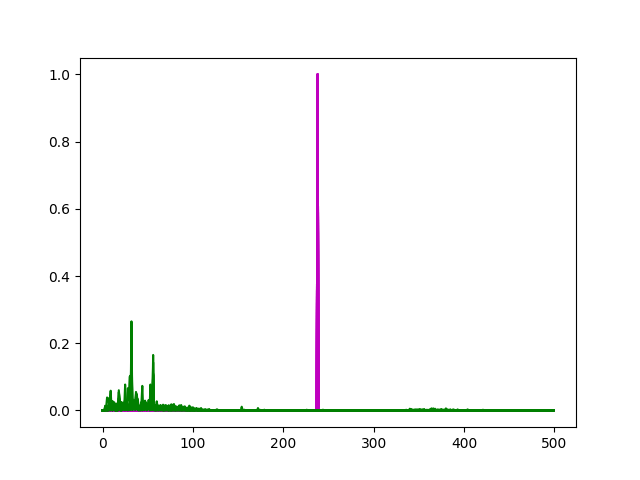
\includegraphics[width=\linewidth]{fake_length_dist}
\caption{Normal vs. FTE fixed width}
\label{fig:fake_length_dist}
\end{subfigure}
\begin{subfigure}[b]{.49\linewidth}
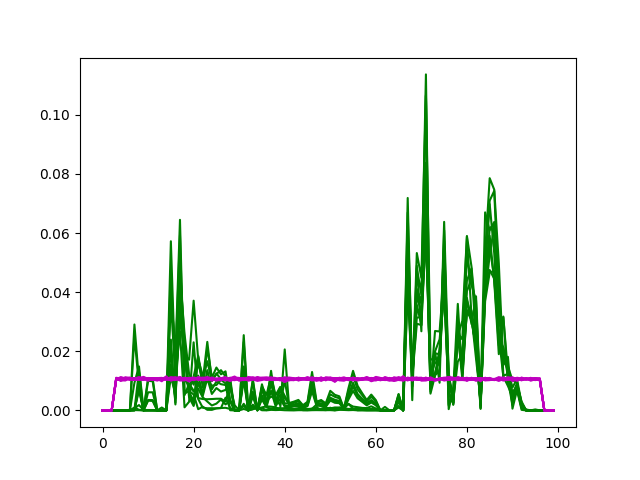
\includegraphics[width=\linewidth]{uniform_length_dist}
\caption{Normal vs. random width}
\label{fig:uniform_length_dist}
\end{subfigure}
\caption{Length Distrbutions}
\end{figure}

In this case, the probability of the packet being exactly 256 bytes is overwhelmingly greater for the FTE scheme than for normal traffic.
Of course, legitimate packets may also be this length so filtering them all out would give false positives.
This might be okay if when the TCP layer re-sent the replacement for the missing, blocked data it would be of a different length and would be let through but in fact it sends an exact copy each time.
Therefore, to amplify the probability of not catching false positives, the system must take a sample from the stream and check them all as a batch.
This could be done on a small running window basis and when triggered could add the IP address to a temporary ban.
This is like what happens in currently deployed keyword filtering systems such as in China. 

Another heuristic for defining the distribution is pattern frequency.
This can be done at varying levels of granularity to give varying results.
The obvious level of abstraction is at the character level, which if used to base an emulation from, will only produce strings containing valid characters, since they are are what is extracted from normal traffic.
Since patterns are recorded and generated independently, any lower level of granularity could produce byte values for non valid characters such as control characters.
This makes detection easy for a censor, as these values are not allowed in the protocol, so they can reject without even considering their frequency of use in normal traffic.
Longer patterns have pros and cons; more character dependence, leading to more realistic URLs to the eye, but the complexity is increased dramatically, as per our exponential calculation previously.
If multiple character patterns are used, sequences of semantically correct content appear such as words and data structures like query string parameters.
I will evaluate the difference in granularity in section \ref{sec:gran}.

Other more less specific specific heuristics include \texttt{inter-slash-distance} and ways to sample pattern distribution from only a subset of the URL such as the \texttt{initial-pattern} or \texttt{random-pattern}. These less powerful measures can all be dealt with in the same way to parametrise an encoding.

\subsection{Detection}

For less obvious differences in heuristic values between normal and fake distributions more comprehensive comparison of the distributions are needed.

For testing distributions that are know to follow fixed-shape but parametrised models, such as a Gaussian, the Z-test can be used by testing the difference in means test statistic.
The T-test is more appropriate for small sample sizes, where the population's standard deviation is hard to estimate since the Z-test relies on this to calculate the significance level.
Although, due to the central limit theorem, these measures could be used, the arbitrary structure of the distributions in question it could result in false positives in the measurements if only the means of the samples were taken in to consideration.

An exact test, such Fisher's exact test, will calculate the exact probability of obtaining each observation in the sample.
Assuming the independence of the observations the overall probability can then be computed and then compared with a significance level threshold.
However, in this situation, the independence assumption is unfounded and furthermore, the computational cost of this method is large, so for large sizes of our samples, other tests are recommended.

The Chi-square test and G-test are more appropriate for these large observation counts. In both of these tests, a test statistic is calculated and its value is then compared with the chi-square distribution to estimate the probability of obtaining that value. 
The subtle difference between them, is that the Chi-square test's statistic is the squared differences of each frequency bin, whereas the G-test calculates the sum of log differences.
Therefore, the chi-squared test penalises a larger difference more heavily that multiple smaller ones, whereas the G-test forgives these large differences by a log scale, so the opposite is true.

There is also a class of tests that measure the divergence between two distributions.
These are not distance measurements since they do not obey the triangle inequality however, they are useful for binary comparison.
The divergence calculation, that Kullback and Leibler outline in their foundational paper, is a measure of entropy between distributions~\cite{dist}. 
This measurement deals with the Shannon Entropy of the systems and quantifies the information gain needed to transform from one distribution to the other and is actually related to the G-test by,
$$G = 2 \Sigma_i O_i \cdot \ln{\frac{O_i}{E_i}} = 2N \Sigma_i o_i \cdot \ln{\frac{o_i}{e_i}}$$,
where $O_i$ and $E_i$ are the observed and expected frequencies when $N$ observations is made and $o_i$ and $e_i$ are the observed and expected proportions.
However, it does have problems in application, such as asymmetry and possible infinite values.
In response to this, Jensen and Shannon took a different tack for their divergence measure, which instead measures the similarity between the distributions. This measure is symmetric and since it measures shared information it can only produce finite values.



\subsection{Sampling Methods}

\subsubsection{Rejection sampling}

Rejection sampling is a technique for generating observations from a given distribution. 
It works by first sampling over the two dimensional space of the proposed frequency density distribution and rejecting those that do not lie below the line.
A classic, well-known, real-life example of this is the Buffon Needle experiment, in which the participant randomly drops needles on to a sheet of paper with evenly distributed parallel bars drawn across it.
The needles that overlap a bar are counted verses those who don't and this proportion can be used to estimate pi as $\pi \approx \frac{2l}{t \cdot P}$ where $l$ is the length of the needles, $t$ is the gap between bars and $P$ is the proportion.
In this case, the first distribution is 3 dimensional; two spatial dimensions and one angular, and the second mapped distributions is binomial.
The transformation formula uses some elementary calculus and involves $pi$, so by knowing the outcome of the experiment, one can work backwards to estimate its value.
However, the major downfall of this method is that the efficiency is greatly affected by the closeness of the two distributions, as more samples have to be rejected.

\subsubsection{Inverse Transform Sampling}

Another more efficient sampling method is called inverse transform sampling, which is commonly used for generating random numbers from arbitrary distributions.
It is simple and efficient and can be used to generate values from the Normal distribution when given values from the uniform sources that are gathered by computer's random generation implementation.
It works by generating samples of a different distribution and then transforming them using a formula.
However, it works by calculating the inverse of the cumulative frequency distribution function so only works on distributions where this is invertible.

\subsubsection{Fully Connected Neural Networks}

Fully connected neural networks with a single hidden layer are theoretically able to model any continuous function.
Therefore, they should be able to convert distributions.
To test this, in early 2018, Horger et al. wrote a paper on training neural nets to generate samples from arbitrary distrobutions~\cite{deepl}.
They trained the fully connected neural net to map uniformly generated inputs to a chosen probability density function by minimising Jensen-Shannon divergence.
Their model was able to produce results that have comparable goodness of fit to other classical methods and after training was competitive in performance.
Large amounts of data are needed to train the system which to be done with realistic performance, needs special hardware to cope with the parallelism. Although, in the not so distant future this may become ubiquitous. 

\subsection{The Proposed Scheme}

My proposed scheme works by generating encoded ciphertexts from a heuristic which can take a finite number of discrete values $\mathcal{H}$. For this, the scheme will use an inverse transform sampling due to its efficiency and ease of computation.
The heuristics follow a distribution $D_n$ defined by a frequency histogram, like shown in figure \ref{fig:dist_pat4}.
Since this is discrete, forming the cumulative distribution is simply the case of iteratively adding the bin frequencies and linearly interpolating the intervals as shown in figure \ref{fig:cum_dist_pat4}.
Since we have a finite number of intervals, the inverse can simply be the reverse lookup function $\mathcal{F}^{-1}_{D_N} :: [0,1) \rightarrow \mathcal{H}$.
Now, assuming our input is uniformly random, sampling over the observations and applying this inverse transform $\mathcal{F}^{-1}_{D_N}$ will obtain values for our heuristics that are normally distributed.
These values can then be used in the encoding to produced normally distributed ciphertexts.

\begin{figure}[h]
\centering
\begin{subfigure}[b]{.49\linewidth}
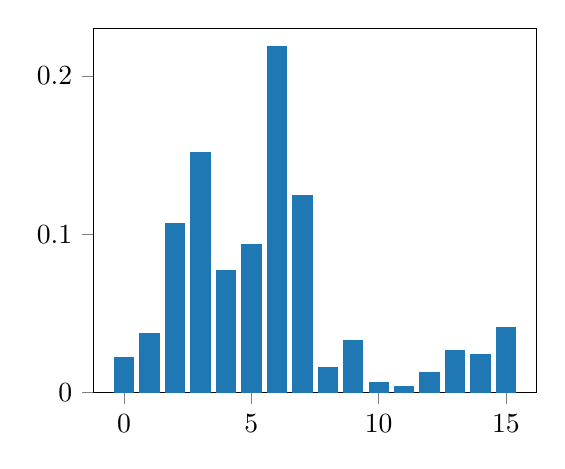
\begin{tikzpicture}

\definecolor{color0}{rgb}{0.12156862745098,0.466666666666667,0.705882352941177}

\begin{axis}[
xmin=-1.19, xmax=16.19,
ymin=0, ymax=0.230154666496227,
tick align=outside,
tick pos=left,
x grid style={lightgray!92.02614379084967!black},
y grid style={lightgray!92.02614379084967!black}
]
\draw[fill=color0,draw opacity=0] (axis cs:-0.4,0) rectangle (axis cs:0.4,0.0223230918645563);
\draw[fill=color0,draw opacity=0] (axis cs:0.6,0) rectangle (axis cs:1.4,0.0376200159943381);
\draw[fill=color0,draw opacity=0] (axis cs:1.6,0) rectangle (axis cs:2.4,0.107301002218318);
\draw[fill=color0,draw opacity=0] (axis cs:2.6,0) rectangle (axis cs:3.4,0.152103855633172);
\draw[fill=color0,draw opacity=0] (axis cs:3.6,0) rectangle (axis cs:4.4,0.0772054181209926);
\draw[fill=color0,draw opacity=0] (axis cs:4.6,0) rectangle (axis cs:5.4,0.0936454073957445);
\draw[fill=color0,draw opacity=0] (axis cs:5.6,0) rectangle (axis cs:6.4,0.219194920472597);
\draw[fill=color0,draw opacity=0] (axis cs:6.6,0) rectangle (axis cs:7.4,0.12484703270733);
\draw[fill=color0,draw opacity=0] (axis cs:7.6,0) rectangle (axis cs:8.4,0.0158984655724211);
\draw[fill=color0,draw opacity=0] (axis cs:8.6,0) rectangle (axis cs:9.4,0.0335779770747821);
\draw[fill=color0,draw opacity=0] (axis cs:9.6,0) rectangle (axis cs:10.4,0.00645483002508274);
\draw[fill=color0,draw opacity=0] (axis cs:10.6,0) rectangle (axis cs:11.4,0.00427860235051296);
\draw[fill=color0,draw opacity=0] (axis cs:11.6,0) rectangle (axis cs:12.4,0.0128734155706284);
\draw[fill=color0,draw opacity=0] (axis cs:12.6,0) rectangle (axis cs:13.4,0.0269999937643906);
\draw[fill=color0,draw opacity=0] (axis cs:13.6,0) rectangle (axis cs:14.4,0.0244379377592649);
\draw[fill=color0,draw opacity=0] (axis cs:14.6,0) rectangle (axis cs:15.4,0.041238033475869);
\end{axis}

\end{tikzpicture}
\caption{Probability Density Function}
\label{fig:dist_pat4}
\end{subfigure}
\begin{subfigure}[b]{.49\linewidth}
\begin{tikzpicture}

\begin{axis}[
xmin=-0.75, xmax=15.75,
ymin=-0.0265607535422159, ymax=1.04888384540677,
tick align=outside,
tick pos=left,
x grid style={lightgray!92.02614379084967!black},
y grid style={lightgray!92.02614379084967!black}
]
\addplot [semithick, black, forget plot]
table {%
0 0.0223230918645563
1 0.0599431078588944
2 0.167244110077212
3 0.319347965710384
4 0.396553383831377
5 0.490198791227121
6 0.709393711699718
7 0.834240744407048
8 0.850139209979469
9 0.883717187054251
10 0.890172017079334
11 0.894450619429847
12 0.907324035000475
13 0.934324028764866
14 0.958761966524131
15 1
};
\end{axis}

\end{tikzpicture}
\caption{Cumulative Probability Density Function}
\label{fig:cum_dist_pat4}
\end{subfigure}
\caption{4-Bit Pattern Length Distributions}
\label{fig:cum_conv}
\end{figure}



\subsection{Invertibility}\label{invertibility}

To map the discrete input, un-encoded ciphertext values onto the continuous domain of $F^{-1}_{D_N}$ some quantisation must be done.
However, the actual distribution structure does have an effect on the degree of quantisation (or more simply put, the amount of splitting) which can be done.
Let $s$ be the number of splits of the continuous space $[0,1)$ and so $d = \frac{1}{s}$.
To ensure that the encoding is invertible, as all encodings must be, we must ensure that our discrete version of $\mathcal{F}^{-1}_{D_N}$: $F^{-1}_{D_N}$ is injective and surjective.

Define:

$$F^{-1}_{D_N} :: \mathbb{Z}_s \rightarrow \mathcal{H}$$
$$F^{-1}_{D_N}(x) = x' \xleftarrow{\$} [x, x+d); \mathcal{F}^{-1}_{D_N}(x')$$

Surjectivity of $F^{-1}_{D_N}$ follows from the fact that $\mathcal{F}^{-1}_{D_N}$ is surjective by, $\forall y \in \mathcal{H}, \exists x' \in [0,1)\ st.\ \mathcal{F}^{-1}_{D_N}(x') = y$ and $ let\ x = \lfloor \frac{x'}{d} \rfloor$ so $x \in \mathbb{Z}_s$ and $F^{-1}_{D_N}(x) = y$ so surjective.

However, injectivity is not provable in general. It depends on the exact instance of the distribution histogram.
In fact, it is very unlikely for no overlaps between output quantisation and input quantisation to occur.
Therefore, I made a tweak to make the system usable.
This was to shrink the input divisions slightly so that they matched up to the nearest output division.
This preprocessing step is outlined in implementation.
It is important to note that if a correction makes the lower bound greater than the higher bound the process is invalid and the splitting rate must be reduced.

\begin{figure}[h]
\centering
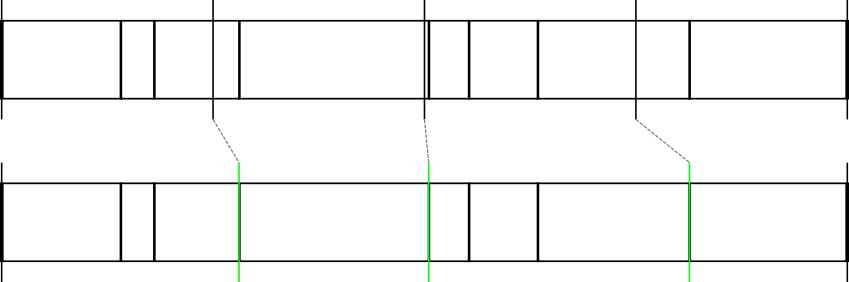
\includegraphics[scale=.9]{correction}
\caption{Showing how the input splitting is corrected to create an injective function.}
\label{correction}
\end{figure}

In the diagram in figure \ref{correction} the smaller lines represent the output histogram boundaries and the longer lines represent the splitting of the input to the function $F^{-1}_{D_N}$.
The green lines are the corrected splittings to force the function to be injective. This preprocessing creates an array of boundaries $B$. Augment $B$ by setting $B = [0] + B$

Redefine:
$$F^{-1}_{D_N}(x) = x' \xleftarrow{\$} [B[x], B[x+1]); \mathcal{F}^{-1}_{D_N}(x')$$

This new function still is surjective by roughly the same proof as before but it's injectivity also holds.
Proof:
Firstly, the correction of the boundaries of the inputs were moved to match the boundaries of the outputs.
The divisions started as non-overlapping and during the correction, this did not change, 
$$\forall i \neq j \in \mathbb{Z}_s, \big[ B[i],B[i+1] \big) \cap \big[ B[j],B[j+1] \big) = \emptyset$$
Also since the boundaries match, the pre-image of a output value is contained by only one input value,
$$ \forall i \neq j \in \mathbb{Z}_s, \alpha,\beta \in \mathcal{H} \text{ such that } \alpha \in Img_{F^{-1}_{D_N}}(\big[ B[i],B[i+1] \big)) \text{ and } \beta \in Img_{F^{-1}_{D_N}}(\big[ B[j],B[j+1] \big))$$
$$\text{ then } \alpha \neq \beta$$
Therefore, if we take arbitrary $x, x' \in \mathbb{Z}_s, \text{ such that letting} \alpha = F^{-1}_{D_N}(x), \text{ and } \beta = F^{-1}_{D_N}(x'), \text{ then } \alpha = \beta \in \mathcal{H}$ then by the contrapositive above $x=x'$.

\subsection{Towards a Concrete Scheme}

The two most promising heuristics for encapsulating the traffic's distribution are length and pattern frequency.
I am targeting length to demonstrate the advantage of my scheme over FTE. Pattern frequency over the whole ciphertext will also fool statistical analysis looking for the more specific heuristics that I mentioned earlier such as \texttt{inter-slash-distance} and \texttt{initial-pattern}.
Therefore, I chose to encapsulate both of these in my scheme. 

A simplification I have made is, like the FTE scheme, to restrict the encoding to only worrying about the path of a HTTP GET request.
The scheme cannot work on the packet as a whole since the pattern independence of the scheme would not be able to produce the correct legal formatting.
Instead, each field of the protocol needs to be dealt with individually according to it's own distribution or heuristic and combined using a formatting algorithm like a regular expression.
It could also be possible for there to be heuristics to decide whether fields such as \texttt{Cookies} should be included at all.
However, each heuristic would be dealt with in the same way, so to limit the scope of the project to a proof of concept, I will only target the path field.
The mechanics of the scheme will use the same structure as FTE. First, an authenticated encryption scheme is used to encrypt the original data using a symmetric key.
This is then passed to the emulator encoding module, which uses the length and pattern heuristic distributions to produce normally distributed ciphertexts.
The un-distributed encryption is constructed from a IV, encrypted blocks, and a HMAC. Therefore, over a choice of random encryption and signing keys it is indistinguishable from random.
Therefore, no matter what the underlying data is the unform distributions that our encodings rely on is upheld. 
The inverse operation must use the same key and heuristic distributions, so can invert each encoding layer and then decrypt using a standard cipher.
I refer to this scheme as DE-CENSOR: a Distribution Encoding of Ciphertexts to Emulate Normal Surfing while Onion Routing.

\subsubsection{Pattern Encoding}

The mechanics of the pattern encoding is basically a base transformation from base 0x100 (characters) to a base of the number of divisions of the pattern heuristic distribution.
Once this new list of digits is produced, the scheme can apply our discrete inverse transformation function $F^{-1}_{D_N}$ to each one to map this to a list of output patterns which can be joined to form the normally pattern-distributed ciphertext.

The un-encode mechanism splits the string of patterns up and then can apply the forward transformation function. The bases of the digits can then be changed back to the byte before forming the original character string once more.

\subsubsection{Length Encoding}

If length encoding took in arbitrary length ciphertexts, it would need to include the length of the original in to the encoding, such as pre-pending the data with it's length as a number of bytes.
However, whatever way this is done, the resulting output will not satisfy the uniform random requirement for the next level (pattern encoding).
To counter this, another level of encryption could be done with another set of keys. However, this is undesirable due to the increased ciphertext length expansion and computational work.
Another solution is to fix the whole scheme to only work on fixed sized blocks as input. TO enforece this messages can be padded before encryption using a secure padding scheme such as defined in ISO 10126~\cite{iso-pad}.


\subsection{Formalising the Scheme}

\subsubsection{Encryption}

The DTE is an encrypt-then-encode framework. To ensure the same standards of encryption as in the FTE scheme DTE must also provide IND-CCA security. To ensure this I will use an authenticated encryption scheme i will use counter mode with HMAC using AES256 for encryption and SHA256 for authentication. Therefore, assuming the underlying block cipher - AES - is secure, this mode provides indistinguishability under a chosen ciphertext attack. This security guarantee is only for the encryption layer. 

TODO: Now prove the property holds for the whole scheme

\subsubsection{Distinguishably}

\begin{itemize}
\item Adversary classifications from 'the parrot is dead'
\item closeness of distributions
\end{itemize}

\section{Implementation}

I have implemented the code for the censor and the de-censor scheme. The censor implementation consists of a measurement program that calculates the statistical similarity of batches of paths to a pre-recorded reference histogram of normal traffic. It compares the statistic to a threshold pre-calculated to separate normal from malicious requests. The de-censor scheme takes in messages, encrypts them and then encodes them using the selected emulator, that outputs an expanded ciphertext but one that is distributed according to it's reference histogram. This can be the same reference distribution as the censor, but a high success rate is also possible using a separately recorded histogram of the same normally distributed background traffic. This is important since practically, it would not be possible to extract the used distribution from in-use instances of the tool.


All the code was written in \texttt{python2.7} for quick prototyping but for performance gains the core could be re-written in \texttt{C/C++} to remove the overheads of the python interpreter. I conducted my implementation and testing on Ubuntu 16.04 on VMware virtual machines running on a low powered i5 Intel VT enabled laptop.

\subsection{Collection}

Packet collection is used for both parties, since both the emulator and censor need to record a reference distribution to work against and the censor is also required to read the packets for classification. Since both my censor and de-censors are running on Ubuntu machines I used the PyShark a python wrapper around the Tshark non-interactive command-line tool. Tshark is also able to parse and filter the packets like currently deployed DPI systems. I used this feature to extract the packets I cared about using the filter in figure \ref{fig:filter}.

\begin{figure}[h]
\begin{verbatim}
http && http.request.method == "GET"
\end{verbatim}
\caption{Tshark packet filter}
\label{fig:filter}
\end{figure}

The filter shows that we only targeted GET requests. This is because HTTP is a very one sided protocol with most of the content moving from the web server to the client and therefore it is harder to hide messages inside the requests. The response encoding should be more straight forward. GET requests as opposed to POST requests take up a larger proportion of web traffic and so are the obvious choice. 

In this experiment I have fixed all other parameters apart from path. This is a proof of principle
of the sides of communication to forge due to it's normally low data size. Files returned from servers are usually much less structured 

To collect real web traffic data, I built a web-crawler using the FOSS Selenium web automation framework. To gather a realistic distribution I needed to emulate the whole browser environment since X amount of the requests from modern sites are dynamics initiated from inside the scripts.
% graph

I crawled recursively over the Alexa top 50 sites~\cite{alexa} that support unencrypted traffic. This gave me a sample of 10,000 paths to create reference distribution.

\subsection{Histogram creation}

Like the recording of reference material, the calculation of distribution histograms is not time critical since they can be done offline. The process is straightforward frequency binning to count the occurrences of each option. I tried several methods as explained below.


\begin{figure}[h]
	\centering
	\begin{subfigure}[b]{0.24\textwidth}
		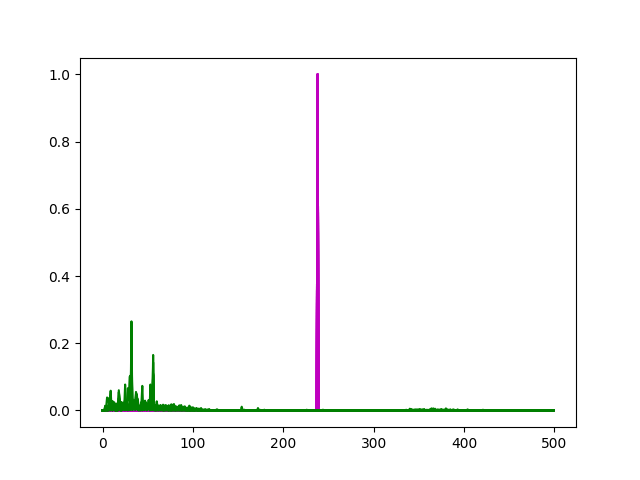
\includegraphics[width=\textwidth]{bob}
		\caption{Path length}
		\label{fig:length_hist}
	\end{subfigure}
	\begin{subfigure}[b]{0.24\textwidth}
		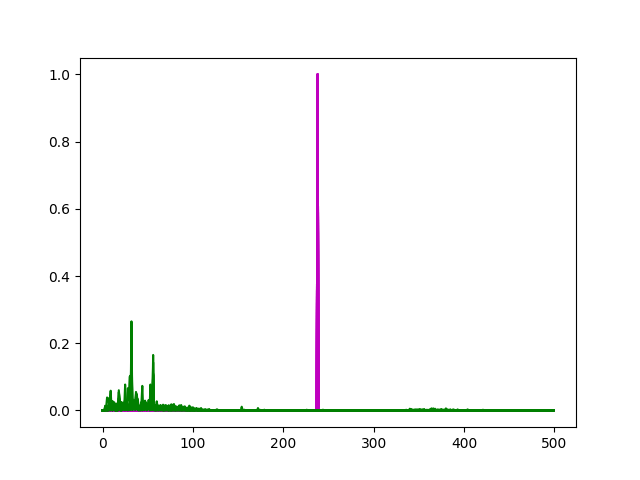
\includegraphics[width=\textwidth]{bob}
		\caption{Character based}
		\label{fig:char_hist}
	\end{subfigure}
	\begin{subfigure}[b]{0.24\textwidth}
		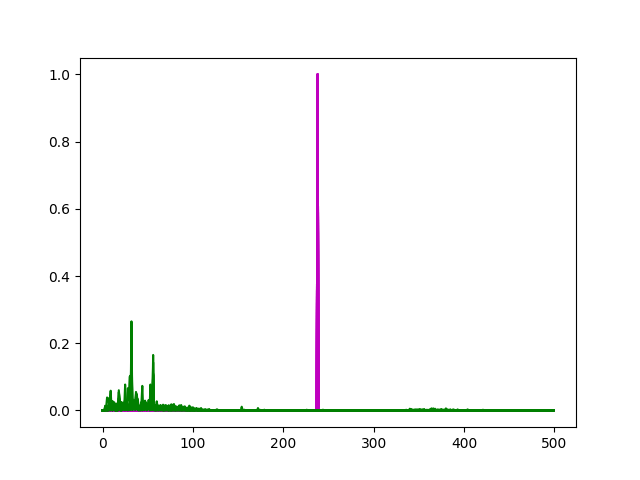
\includegraphics[width=\textwidth]{bob}
		\caption{First Letter}
		\label{fig:first_hist}
	\end{subfigure}
	\begin{subfigure}[b]{0.24\textwidth}
		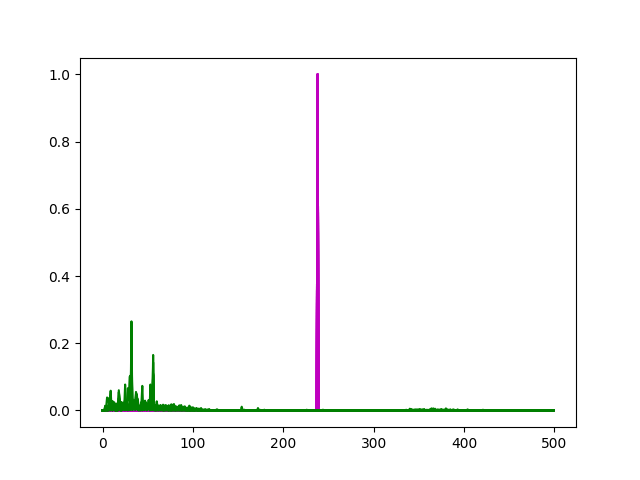
\includegraphics[width=\textwidth]{bob}
		\caption{Random Letter}
		\label{fig:rand_hist}
	\end{subfigure}

	\caption{Distribution Histographs}\label{fig:hists}
\end{figure}

\textbf{Path length} - this was targeted at the FTE scheme that used a fixed length. It shows very few examples would be needed to differentiate the origins.

\textbf{Character distribution} - This graph exibits the underlying encryption schemes uniform randomness, whereas in real traffic not all characters are created equally.

\textbf{First Letter} - This method was attempted to see if the same distinguishing effect would be possible only using a fixed subset of the URL.

\textbf{Random Letter} - like the previous this uses a limited sample by randomises it's location to see if this improved on the above results.

\subsubsection{Exponential Scaling}

As the length of the patterns increase, the number of frequency bins increases exponentially, and therefore, if they are backed by an fully allocated array the space needed to record the frequencies quickly becomes unmanageable.
For instance, even at pattern size of four characters it will consume 4 GiB in memory.
Next, we observe that very little of the large space containing the all the possible patterns is ever used, since the samples collected are very small in comparison.

Therefore, instead of allocating giant chunk of contiguous memory, the system will use a hash table.
This dynamic structure handles the allocation of memory to match the number of items actually stored.
Since we can estimate the expected number of items to be used during the analysis, we can also pre-resize the hash table to avoid the expensive operation of resizing in operation to avoid collisions.

\subsection{Inverse Transform Function}

As described in section \ref{invertibility}, the inverse transform function $F^{-1}_{D_N}$ maps values drawn from uniform random to values that have a distribution defined by a frequency histogram.
To implement this, I first transformed this in to a cumulative frequency distribution, and then extracted the upper and lower bounds for each of the output bins which represent each heuristic value.
Then, sampling consists of sampling uniformly over the range of the whole cumulative distribution, and finding in to which bin's bounds the value falls.

This can be done by linear search but as the number of bins grows, this dominates the computation.
Since the bounds are ordered we can replace the lookup with a binary search whose logarithmic complexity slows the increase of computational work.

\subsection{Thresholding}

The detection system's goal is to decide whether a sample of packets is from normally distributed traffic or from a stream of fake ciphertexts such as that is generated from an FTE proxy.
It does this by calculating a corresponding statistic value for the batch of packets in question and applying a threshold to obtain the binary decision.
The threshold is the point that has equal probability of belonging to each distribution and to calculate this, the distribution types and parameters must be decided.
By the central limit theorem, we can model the statistic's value as belonging to a Gaussian distribution, that parameters of which can be estimated from a sample.
I took a sample of 10 streams of normal and fake traffic to get examples from each population and calculated the sample mean and variance. I was then able to estimate the population mean and variance and construct the following equation to constrain the threshold's value.

$$(\sigma_2-\sigma_1) x^2 + 2\cdot (\sigma_1*\mu_2 - \sigma_2*\mu_1) x +  (\sigma_2*\mu_1^2 - \sigma_1*\mu_2^2 - \sigma_1*\sigma_2*\log(\sigma_2/\sigma_1)) = 0$$

This can be solved for x using the standard quadratic formula to obtain the statistic threshold.

\subsection{Proxy Embedding}

I embedded the DE-CENSOR scheme inside the same proxy framework as FTE.
This enables point to point innocuous channel communication using a client-server model.
A user runs a client application on their machine, which listens on a local port.
Any application can then use this port as a SOCKS proxy, which channels the traffic through the innocuous channel to the server.
The server, decodes and unencrypts the data and follows then SOCKS protocol to forward the traffic on to it's ultimate destination.
The keys and distributions must be pre-shared to allow the original traffic to be recovered, though I've included an example distribution as the default.
The encoding happens inside a custom DE-CENSOR record layer which works on a series of buffers to transform the data before it is sent.

\subsubsection{Encoding}

\begin{enumerate}
\item Firstly, data is placed into a plaintext buffer as it arrives.

\item The encryption stage then consumes a fixed length block of the plaintext from the plaintext buffer and produces a ciphertext.
This is placed in the encrypted-buffer.

\item The length encoding stage then transforms these encrypted fixed length messages in to blocks of normal distributed lengths for the length-buffer.

\item Each length of message is then picked by the pattern encoder one at a time, where it undergoes the final transformation in to a normally distributed GET-request paths. 

\item These paths are wrapped into a HTTP GET packet which is then sent across the network over a unencrypted TCP channel to the listening proxy server.
\end{enumerate}

\subsubsection{Decoding}

\begin{enumerate}
\item As the server receives them, HTTP packets are placed into a packet-buffer.

\item The path of each packet is then extracted and fed into the pattern decoder, which reverses the pattern encoding according to the pattern distribution.

\item The length encoding stage then joins the messages back in to strings of fixed equal length.

\item The decryption stage then deciphers the ciphertexts and removes the padding to recover the original messages.

\item The SOCKS protocol headers are then used to pass on the original requests to the intended address.

\end{enumerate}

See figure \ref{fig:imp-diag} for an overview of the process.

\begin{figure}[b]
\begin{subfigure}{\textwidth}
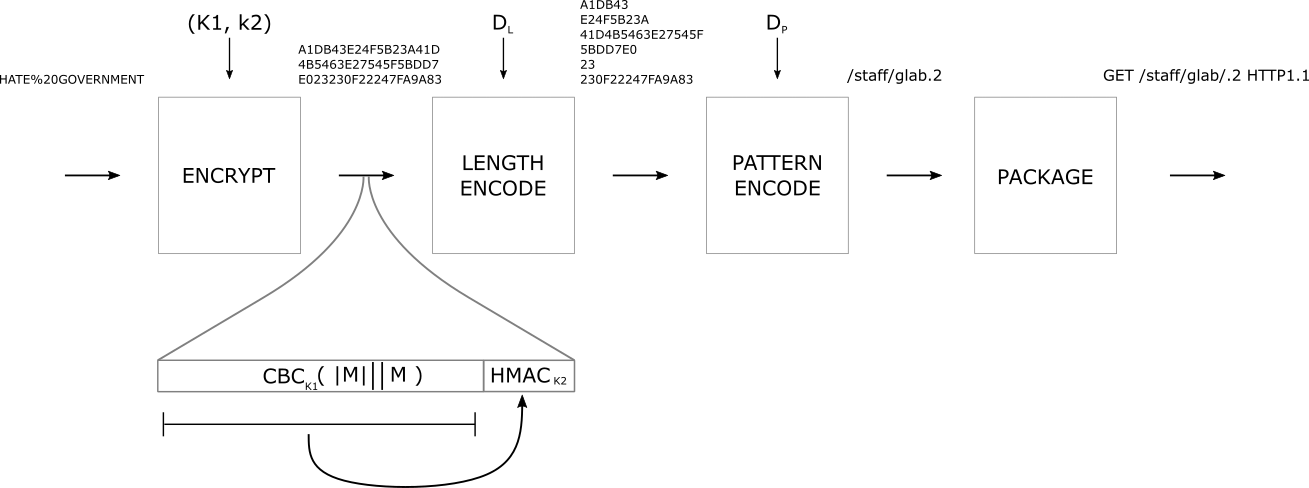
\includegraphics[scale=0.9]{diagram-enc}
\caption{Encoding and Sending Mechanism}
\end{subfigure}

\begin{subfigure}{\textwidth}
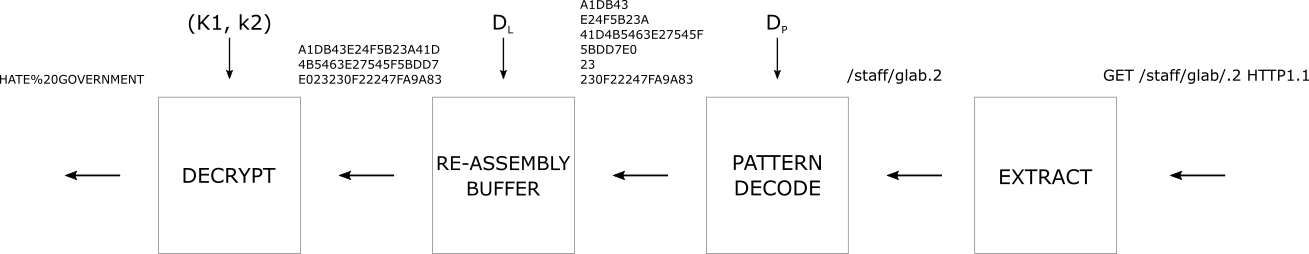
\includegraphics[scale=0.9]{diagram-dec}
\caption{Receiving and Decoding Mechanism}
\end{subfigure}
\caption{Implementation Diagrams}
\label{fig:imp-diag}
\end{figure}

\subsection{Libraries}

I used the Cryptography implementation from the PyCrypto library.This provides an AES block cipher, SHA256 Hash in a Merkle-Damg$\mathring{a}$rd construction and counter mode framework. The IV is chosen randomly.

The statistical distribution comparison calculations are done by the SciPy Library, which provides a C++ back-end to complete the heavy lifting and improves the performance.

% -----------------------------------------------------------------------------

\chapter{Critical Evaluation}
\label{chap:evaluation}

\section{Evaluating Pattern Length Effects}\label{sec:gran}

\begin{table}[h]
\centering
\begin{tabular}{|c|c|c|c|c|c|c|c|c|c|}
\hline
\multirow{2}{*}{Pattern Length}&
\multicolumn{3}{|c|}{Distrobution Bin Number}&
\multicolumn{3}{|c|}{Max Splitting}&
\multicolumn{3}{|c|}{Extension Factor}\\
\cline{2-10}
&10000&20000&30000&10000&20000&30000&10000&20000&30000\\
\hline
4 	& 16&16&16 				& 5&5&6 		& 1.7&1.7&1.6\\
8 	& 81&82&89 				& 14&14&19		& 2.1&2.1&1.9\\
16 	& 3310&3906&5184 		& 52&68&51 		& 2.8&2.6&2.8\\
24 	& 10115&16443&63273 	& 101&88&100 	& 3.6&3.7&3.6\\
32 	& 16471&28031&97963 	& 93&88&95 		& 4.9&5.0&4.8\\
40 	& 19464&33393&105573 	& 88&95&99 		& 6.2&6.1&6.0\\
48 	& 19863&34881&104888 	& 80&69&152 	& 7.6&7.9&6.6\\
\hline
\end{tabular}
\caption{Effects of changing Pattern length}
\label{tab:patlen}
\end{table}

Table \ref{tab:patlen} shows some trends that occur when the pattern length is altered. The statistics are gathered from analysis of one reference sample of normal URLs.

\begin{figure}[h]
\centering
\begin{subfigure}[b]{.49\linewidth}
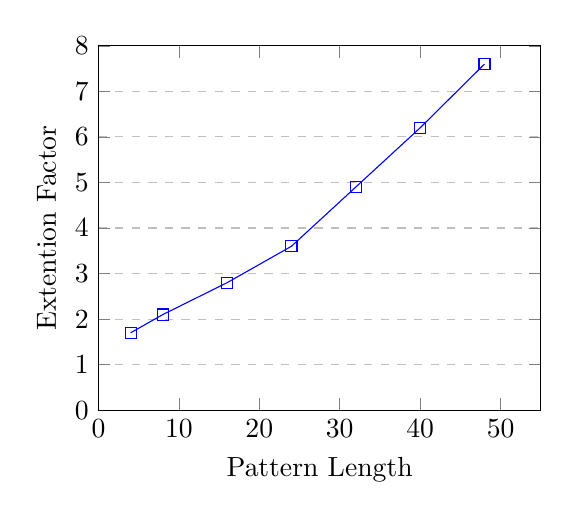
\begin{tikzpicture}

\begin{axis}[
    ylabel={Extention Factor},
    xlabel={Pattern Length},
    xmin=0, xmax=55,
    ymin=0, ymax=8,
    ytick={0,1,2,3,4,5,6,7,8},
    xtick={0,10,20,30,40,50},
    legend pos=north west,
    ymajorgrids=true,
    grid style=dashed,
]
 
\addplot[color=blue,mark=square]
    coordinates {(4,1.7)(8,2.1)(16,2.8)(24,3.6)(32,4.9)(40,6.2)(48,7.6) };
 
\end{axis}

\end{tikzpicture}
\end{subfigure}
\begin{subfigure}[b]{.49\linewidth}
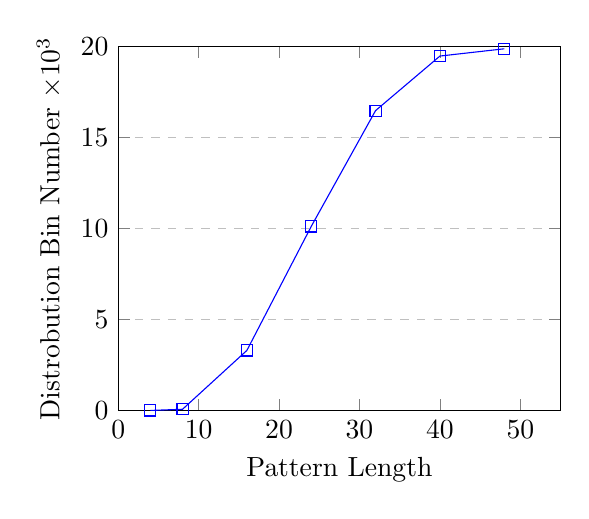
\begin{tikzpicture}

\begin{axis}[
    ylabel={Distrobution Bin Number $\times 10^3$},
    xlabel={Pattern Length},
    xmin=0, xmax=55,
    ymin=0, ymax=20,
    ytick={0,5,10,15,20},
    xtick={0,10,20,30,40,50},
    legend pos=north west,
    ymajorgrids=true,
    grid style=dashed,
]
 
\addplot[color=blue,mark=square]
    coordinates {(4,0.016)(8,0.081)(16,3.310)(24,10.115)(32,16.471)(40,19.464)(48,19.863) };
 
\end{axis}
\end{tikzpicture}
\end{subfigure}
\end{figure}


\begin{wrapfigure}{L}{0.5\textwidth}

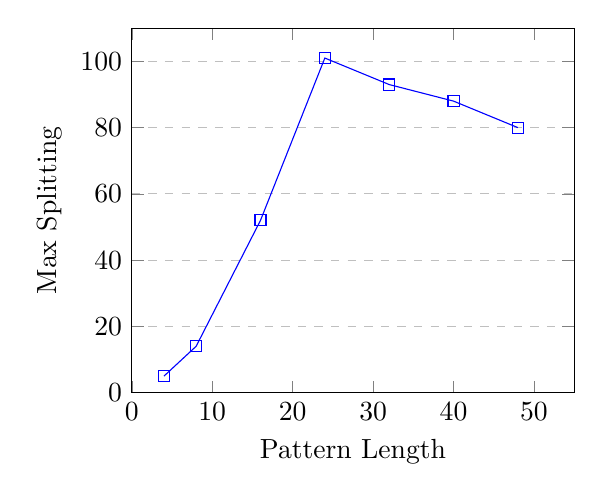
\begin{tikzpicture}
\begin{axis}[
    ylabel={Max Splitting},
    xlabel={Pattern Length},
    xmin=0, xmax=55,
    ymin=0, ymax=110,
    ytick={0,20,40,60,80,100},
    xtick={0,10,20,30,40,50},
    legend pos=north west,
    ymajorgrids=true,
    grid style=dashed,
]
 
\addplot[color=blue,mark=square]
    coordinates {(4,5)(8,14)(16,52)(24,101)(32,93)(40,88)(48,80) };
 
\end{axis}
\end{tikzpicture}
\caption{Pattern Length statistics on sample size $10000$}
\end{wrapfigure}

The expansion factor follows the following equation; let $s$ be the maximum splitting before errors, and $pl$ to be the patten length.
$$|output| = |input| \times \left( \log_s 256 \times pl / 8 \right)$$ 
This stems from the conversion of bases from $0x100=256$ in a character to $s$ divisions over the pattern of $pl$ bits and therefore $pl/8$ bytes. The equation shows the linear correlation between pattern length and expansion, though the graph shows the rate of inefficiency increases slightly with pattern size. This is due to the how well the bigger pattern distributions split in the equal portions. Initially, the splitting amount increases but after 24 bits (3 characters) it pivots and gradually decreases.  This is due to the increasing variance in bin size as the patterns get larger, causing the packing into divisions harder. I will discuss the techniques of packing in the implementation section. 

The distribution bin number describes the number of non-empty bins in the histogram describing the distributions.
At small numbers this is very low, since for sub-byte patterns the unstructured definition of \texttt{ascii} representations means any character distribution tends to produce all patterns of that length.
At the byte length, looking at table \ref{tab:patlen}, it is clear not all character as created equal, since only a maximum of 89 different byte patterns are seen.
In a purely random sample you would expect to see the number of bins used to increase exponentially, however, the graph shows this is not the case as the rate of increase slows.
This could be since as the pattern length increases, the number of patterns in the sample that it has to draw from decreases.
Also, the variation between histogram bin sizes widens since smaller patterns used in different permutations produce even spreading throughout the histogram even if the larger patterns the permutations make up are very uneven.
To give concrete examples, let's take the examples of length 4 and 40.
Length 4 produces 16 bins, of which the maximum proportion is $0.2191$, whereas for length 40 with 105573 bins has a maximum proportion of a smaller absolute value $0.0024$.
However, when we take these are ratios from uniform we get $\frac{0.2191}{\frac{1}{16}} = 0.2191 \cdot 16 = 3.5056$ and $\frac{0.00245}{\frac{1}{105573}} = 0.00245 \cdot 105573 = 258.65385$.
In the case of length 40 the particular value corresponds to the string \texttt{['/', 'i', 'm', 'a', 'g']}, which as expected, is an extremely common string in today's media rich web experiences, especially when to compared to low frequency strings such as \texttt{['V', 'U', 'S', '5', 'W']} which is probably only appearing in cryptographic random identifiers.
For the 4 bit case, the most common result is \texttt{0x6}, which also is expected since the \texttt{ascii} representation of the letters \texttt{[a-o]} are in the range $0x60 \leq x < 0x70$.
To sum up, the smaller the patterns lead to more independence and so more even distributions. 


\begin{figure}[h]
\centering
\begin{subfigure}[b]{.49\linewidth}
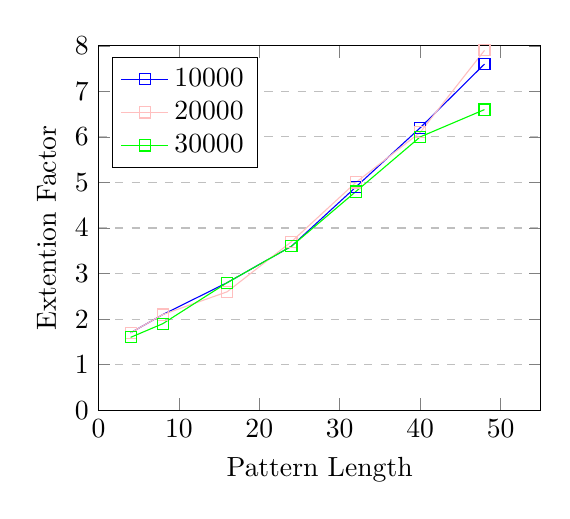
\begin{tikzpicture}

\begin{axis}[
    ylabel={Extention Factor},
    xlabel={Pattern Length},
    xmin=0, xmax=55,
    ymin=0, ymax=8,
    ytick={0,1,2,3,4,5,6,7,8},
    xtick={0,10,20,30,40,50},
    legend pos=north west,
    ymajorgrids=true,
    grid style=dashed,
]
 
\addplot[color=blue,mark=square]
    coordinates {(4,1.7)(8,2.1)(16,2.8)(24,3.6)(32,4.9)(40,6.2)(48,7.6) };
    \addlegendentry{10000}
\addplot[color=pink,mark=square]
    coordinates {(4,1.7)(8,2.1)(16,2.6)(24,3.7)(32,5.0)(40,6.1)(48,7.9) };
    \addlegendentry{20000}
\addplot[color=green,mark=square]
    coordinates {(4,1.6)(8,1.9)(16,2.8)(24,3.6)(32,4.8)(40,6.0)(48,6.6) };
    \addlegendentry{30000}
 
\end{axis}

\end{tikzpicture}
\end{subfigure}
\begin{subfigure}[b]{.49\linewidth}
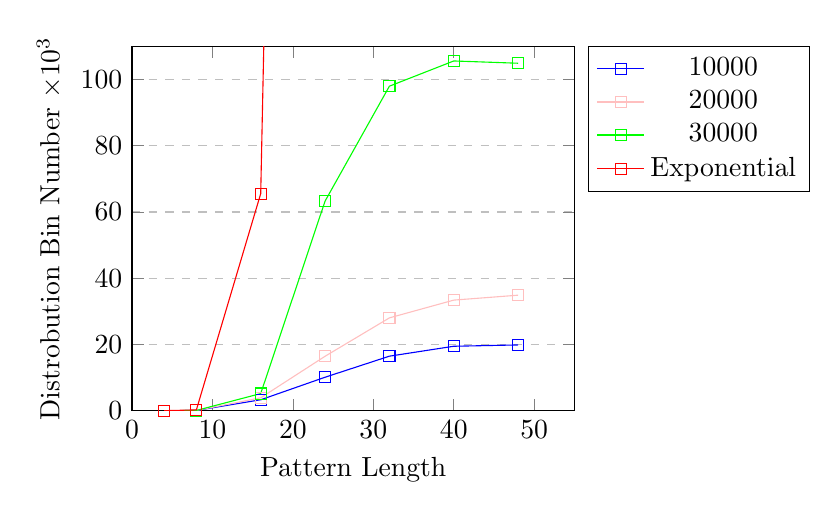
\begin{tikzpicture}



\begin{axis}[
    ylabel={Distrobution Bin Number $\times 10^3$},
    xlabel={Pattern Length},
    xmin=0, xmax=55,
    ymin=0, ymax=110,
    ytick={0,20,40,60,80,100},
    xtick={0,10,20,30,40,50},
    legend pos=outer north east,
    ymajorgrids=true,
    grid style=dashed,
]
 	
\addplot[color=blue,mark=square]
    coordinates {(4,0.016)(8,0.081)(16,3.310)(24,10.115)(32,16.471)(40,19.464)(48,19.863) };
    \addlegendentry{10000}
\addplot[color=pink,mark=square]
    coordinates {(4,0.016)(8,0.082)(16,3.906)(24,16.443)(32,28.031)(40,33.393)(48,34.881) };
    \addlegendentry{20000}
\addplot[color=green,mark=square]
    coordinates {(4,0.016)(8,0.089)(16,5.184)(24,63.276)(32,97.963)(40,105.573)(48,104.888) };
    \addlegendentry{30000}
\addplot[color=red,mark=square]
    coordinates {(4,0.016)(8,0.256)(16,65.536)(24,1000) };
    \addlegendentry{Exponential}
 
\end{axis}
\end{tikzpicture}
\end{subfigure}
\end{figure}

\begin{wrapfigure}[13]{R}{0.5\textwidth}
\centering

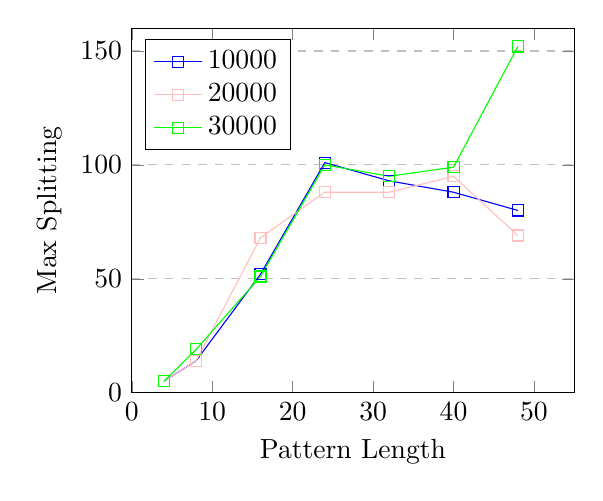
\begin{tikzpicture}
\begin{axis}[
    ylabel={Max Splitting},
    xlabel={Pattern Length},
    xmin=0, xmax=55,
    ymin=0, ymax=160,
    ytick={0,50,100,150},
    xtick={0,10,20,30,40,50},
    legend pos=north west,
    ymajorgrids=true,
    grid style=dashed,
]

\addplot[color=blue,mark=square]
    coordinates {(4,5)(8,14)(16,52)(24,101)(32,93)(40,88)(48,80) };
   	\addlegendentry{10000}
\addplot[color=pink,mark=square]
    coordinates {(4,5)(8,14)(16,68)(24,88)(32,88)(40,95)(48,69) };
	\addlegendentry{20000}
\addplot[color=green,mark=square]
    coordinates {(4,5)(8,19)(16,51)(24,100)(32,95)(40,99)(48,152) };
    \addlegendentry{30000}
 
\end{axis}
\end{tikzpicture}
\end{wrapfigure}

To investigate the effect of the reference sample size on these figures I extracted more network traffic so I had 3 different-sized datasets.

The figure on histogram-bin-numbers shows how although each sample size does have diminishing returns, as pattern length increases, the maximum value reached does improve directly with the size of the sample. This is because although at small pattern sizes the samples are exhaustive, on larger patterns although the actual normal distribution may contain upto an exponential number of sequences in a fixed sample we only ever see a small portion of them. 

I believe the largest sample produces such a large increase compared to the step from 10000 to 20000 due to the way the web crawler worked.
As described in the implementation section, it starts at a small set of sites and ventures outwards by following links on the pages.
Because of this, the number of sites increases but also the diversity of these sites increases in language, style and technologies (different web frameworks produce different request patterns).

On larger samples the possible encoding output expansion is slightly less for larger pattern length than when using a smaller one. This is due to the increase in possible number of divisions of the distribution down to the larger number of bins giving a more evenly divided distribution.


\subsection{Other Solutions}

ObfsProxy simply encrypts the entire packet with a streaming cipher. Earlier versions used a fixed parameters so although expensive, decryption could be done to obtain the standard traffic but now even that is not possible since a key exchange produces ephemeral keys. This procedure produces ciphertexts that are computationally indistinguishable from a random string so intensive computational statistics would be able to differentiate this from a background distribution of standard traffic. Also, do to it's complete lack of structure it would not pass any protocol white-listing filters.

StegoTorus is a system that uses carefully hand crafted embeddings for ciphertexts. In the HTTP mode, it selects randomly for pre-recorded traces and hides the chopped up ciphertext inside Javascript, PDF and SWF files and header fields like Cookies. Since, the masquerading protocol is HTTP, blocking encrypted protocols will not stop this. However, it relies on distributing large volumes of these traces or everyone recording their own, otherwise censors could just block all of them specifically. This means the overhead in communication but mainly storage of traces is large 


meek\\
Description: Is a transport that uses HTTP for carrying bytes and TLS for obfuscation. Traffic is relayed through a third-party server (Google App Engine). It uses a trick to talk to the third party so that it looks like it is talking to an unblocked server.

ScrambleSuit\\
Description: Is a pluggable transport that protects against follow-up probing attacks and is also capable of changing its network fingerprint (packet length distribution, inter-arrival times, etc.).
Language: Python

SkypeMorph\\
Description: It transforms Tor traffic flows so they look like Skype Video. See its source code and design paper.

Dust\\
Description: It aims to provide a packet-based (rather than connection-based) DPI-resistant protocol. See its git repository.


% -----------------------------------------------------------------------------

\chapter{Conclusion}
\label{chap:conclusion}

{\bf A compulsory chapter,     of roughly $5$ pages} 
\vspace{1cm} 

\noindent
The concluding chapter of a dissertation is often underutilised because it 
is too often left too close to the deadline: it is important to allocation
enough attention.  Ideally, the chapter will consist of three parts:

\begin{enumerate}
\item (Re)summarise the main contributions and achievements, in essence
      summing up the content.
\item Clearly state the current project status (e.g., ``X is working, Y 
      is not'') and evaluate what has been achieved with respect to the 
      initial aims and objectives (e.g., ``I completed aim X outlined 
      previously, the evidence for this is within Chapter Y'').  There 
      is no problem including aims which were not completed, but it is 
      important to evaluate and/or justify why this is the case.
\item Outline any open problems or future plans.  Rather than treat this
      only as an exercise in what you {\em could} have done given more 
      time, try to focus on any unexplored options or interesting outcomes
      (e.g., ``my experiment for X gave counter-intuitive results, this 
      could be because Y and would form an interesting area for further 
      study'' or ``users found feature Z of my software difficult to use,
      which is obvious in hindsight but not during at design stage; to 
      resolve this, I could clearly apply the technique of Smith [7]'').
\end{enumerate}

% =============================================================================

% Finally, after the main matter, the back matter is specified.  This is
% typically populated with just the bibliography.  LaTeX deals with these
% in one of two ways, namely
%
% - inline, which roughly means the author specifies entries using the 
%   \bibitem macro and typesets them manually, or
% - using BiBTeX, which means entries are contained in a separate file
%   (which is essentially a databased) then inported; this is the 
%   approach used below, with the databased being dissertation.bib.
%
% Either way, the each entry has a key (or identifier) which can be used
% in the main matter to cite it, e.g., ~\cite{X}, ~\cite[Chapter 2}{Y}.

\backmatter

\bibliography{dissertation}

% -----------------------------------------------------------------------------

% The dissertation concludes with a set of (optional) appendicies; these are 
% the same as chapters in a sense, but once signaled as being appendicies via
% the associated macro, LaTeX manages them appropriatly.

\appendix

\chapter{An Example Appendix}
\label{appx:example}

Content which is not central to, but may enhance the dissertation can be 
included in one or more appendices; examples include, but are not limited
to

\begin{itemize}
\item lengthy mathematical proofs, numerical or graphical results which 
      are summarised in the main body,
\item sample or example calculations, 
      and
\item results of user studies or questionnaires.
\end{itemize}

\noindent
Note that in line with most research conferences, the marking panel is not
obliged to read such appendices.

% =============================================================================

\end{document}
